\documentclass[a4paper,12pt]{article}

% Packages
\usepackage[utf8]{inputenc}  % Input encoding
\usepackage[T1]{fontenc}     % Font encoding
\usepackage[english]{babel}  % Language
\usepackage{graphicx}
\usepackage{amsthm}
\usepackage{amsmath}
\newtheorem{theorem}{Theorem}[section]
\newtheorem{definition}{Definition}[section]
\usepackage{amssymb}

% Title information
\title{Homework 1, Computational Statistics}
\author{Alessio Manetti}
\date{\today}  % Automatic compilation date



\begin{document}

% Title page
\maketitle
\tableofcontents  % Automatically generated table of contents

\newpage

\section{Exercise 1}
We simulate the parameters
\[a \sim U(2.5,5.5), \ \lambda \sim U(2,4)\]
obtaining the values
\[a = 4.706901, \ \lambda = 3.049805.\]
We set the remaining parameters to
\[b = 1, \ p = 0.5.\]
We have a random variable \(Z \in \{0,1\}\) with distribution
\[Z \sim Bern(p)\]
and, conditionally on \(Z\), a random variable \(Y\) with the following distribution
\[Y|Z=0 \sim P(\lambda) \ \ \ \ Y|Z=1 \sim G(a,b).\]

\subsection{Samples from the marginal of \(Y\) and MC estimate of the CDF}
In order to simulate samples from the marginal of \(Y\), we simulate a vector \(z\) of \(n = 1000\) samples from \(Z\) and we create an empty vector \textit{y\_sample}, to be filled afterwards with the observations of \(Y\), a second empty vector \textit{y\_sample\_z0}, to be filled with the observations of \(Y|Z=0\), and a third empty vector \textit{y\_sample\_z1}, to be filled with the observations of \(Y|Z=1\), all of the same length \(n\). \\
Iterating over the number of samples of \(Z\):
\begin{enumerate}
    \item if the generic sample of index \(i\) of \(Z\) takes the value \(0\), then the vectors \textit{y\_sample} and \textit{y\_sample\_z0} are filled at index \(i\) with a sample from \(Y|Z=0 \sim P(\lambda)\), while the vector \textit{y\_sample\_z1} is filled at index \(i\) with the value \(-1\);
    \item if the generic sample of index \(i\) of \(Z\) takes the value \(1\), then the vectors \textit{y\_sample} and \textit{y\_sample\_z1} are filled at index \(i\) with a sample from \(Y|Z=1 \sim G(a,b)\), while the vector \textit{y\_sample\_z0} is filled at index \(i\) with the value \(-1\).
\end{enumerate}
In this way \textit{y\_sample} holds the samples from \(Y\), \textit{y\_sample\_z0} the samples from \(Y|Z = 0\) and \textit{y\_sample\_z1} the samples from \(Y|Z=1\). \\
In order to compute the CDF of \(Y\) we create a vector \textit{y\_seq} of \(n\) equally spaced elements between the minimum and the maximum value of \textit{y\_sample}, and an empty vector \(cdf\) of length \(n\): this vector will be filled with the values taken by the CDF. \\
The CDF of a random variable can be written as
\[ F(a) = \int_{-\infty}^{a} f(x) \ d\lambda(x) = \int_{-\infty}^{\infty} \mathbb{I}\{ x \leq a\} f(x) \ d\lambda(x) = E\left( \mathbb{I}\{ x \leq a\} \right) \approx \frac{\sum_{i=1}^{n} \mathbb{I}\{ x \leq X_i \}}{n}\]
where the \(X_i, \ i = 1,...,n,\) are, in our case, the elements of \textit{y\_seq}. \\
This method yields the following results:
\begin{center}
    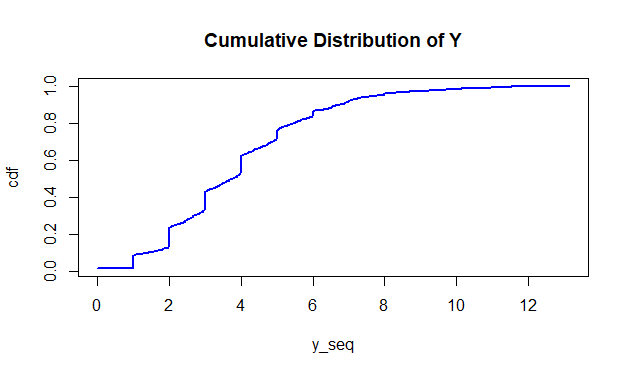
\includegraphics[width = 1\textwidth]{images/Rplot05.png}
\end{center}
where the blue curve is the MC estimate of our CDF.

\subsection{MC estimate of probabilities and variance of the estimator}
 We are asked to compute \( f(Y \in [3.5,4.5]) \) and \(f(Y \in [3.5,4.5]|Z = 0)\). \\
 To this end we use again the MC approximation, which states that
 \[f(Y \in [3.5,4.5]) \approx \frac{\sum_{i=1}^{n} \mathbb{I}\{ y_i \in [3.5,4.5] \}}{n}\]
 and
 \[f(Y \in [3.5,4.5]|Z=0) \approx \frac{\sum_{i=1}^{n^*} \mathbb{I}\{ y_i \in [3.5,4.5]|z = 0 \}}{n^*} = \frac{\sum_{i=1}^{n^*} \mathbb{I}\{ y\_z0_i \in [3.5,4.5]\}}{n^*}\]
 where \(y_i\) is the generic element of \textit{y\_sample}, \(y\_z0_i\) is the generic element of \textit{y\_sample\_z0} and \(n^*\) is the number of observations from \(Y|Z = 0\). \\
 Using this approximation, we obtain the following results:
 \[f(Y \in [3.5,4.5]) \approx 0.186\]
 and
 \[f(Y \in [3.5,4.5]|Z=0) \approx 0.1897959.\]
Now, the variance of the first estimator can be written as
\[ v_{n\_y} = var(\Bar{h}_n) = var\left( \frac{\sum_{i=1}^{n} \mathbb{I}\{ y_i \in [3.5,4.5] \}}{n} \right)\]
which can be approximated by
\[v_{n\_y} \approx \frac{1}{n^2} \sum_{i = 1}^{n} \left( \mathbb{I}\{ y_i \in [3.5,4.5] \} - \Bar{h}_n \right)^2.\]
Analogously, for the second estimator,
\[ v_{n\_yz0} \approx \frac{1}{(n^*)^2} \sum_{i = 1}^{n^*} \left( \mathbb{I}\{ y\_z0_i \in [3.5,4.5] \} - \Bar{h}_{n^*} \right)^2.\]
Using these approximations, we obtain the following results:
\[ v_{n\_y} \approx 0.000151404\]
and
\[ v_{n\_yz0} \approx 0.0003903392.\]

\subsection{MC estimate of probabilities}
We are asked to compute \( f(Z = 0|Y \in [1.5,3.5]) \) and \(f(Z = 1|Y \in [1.5,3.5]) \). \\
In order to answer, we rely on the following:
\begin{theorem}[Bayes]
    Given two random variables \(X\) and \(Y\), then
    \[f(x|y) = \frac{f(x,y)}{f(y)} = \frac{f(y|x)f(x)}{f(y)}\]
    where \(f(y) = \int f(y,x) \ d\lambda(x)\).
\end{theorem}
From this result we deduce that
\[f(Z=0|Y \in [1.5,3.5]) = \frac{f(Y \in [1.5,3.5]|Z=0) f(Z=0)}{f(Y \in [1.5,3.5])}\]
and
\[f(Z=1|Y \in [1.5,3.5]) = \frac{f(Y \in [1.5,3.5]|Z=1) f(Z=1)}{f(Y \in [1.5,3.5])}.\]
All the factors on the right-hand side are easily estimated using what was described in the previous point, so we obtain the following results:
\[f(Z=0|Y \in [1.5,3.5]) = 0.5645161\]
and
\[f(Z=1|Y \in [1.5,3.5]) = 0.4354839.\]

\subsection{Estimation of the empirical quantiles through the generalised inverse}
First of all, we give the following:
\begin{definition}[Generalised inverse or quantile function]
    For a non-decreasing function F on \(\mathbb{R}\), the generalised inverse of \(F\), denoted by \(F^{-1}\), is defined as
    \[F^{-1}(u) = \inf\{x: u \leq F(x)\}\]
\end{definition}
In our case, \(F\) is the CDF computed above. \\
We are asked to compute the empirical quantiles at levels \(0.1,0.2,0.5,0.75\) of \(Y\) and \(Z\), that is
\[ F^{-1}(0.1), \ F^{-1}(0.2),\ F^{-1}(0.5), \ F^{-1}(0.75)\]
where \(F\) is first the CDF of Y, then the CDF of Z. \\
In the first case, for each empirical quantile of level \(u\), we store the index \(i\) of the first value of the vector \textit{cdf} for which the condition
\[u \leq cdf[i] \]
holds. The required empirical quantile is then the value associated with the \(i\)-th index of the vector \textit{y\_seq}. \\
The second case, for \(Z\), is handled in the same way, with the difference that the CDF is built explicitly and takes the following form:
\begin{center}
    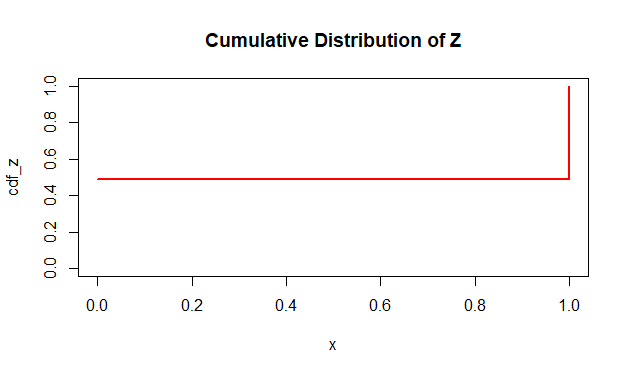
\includegraphics[width = 1\textwidth]{images/Rplot06.png}
\end{center}
We obtain the following results:
\begin{itemize}
    \item for the distribution of \(Y\):
    \begin{center}
        \begin{tabular}{|c|c|c|c|c|}
        \hline
        \textbf{Percentiles} & 0.1 & 0.2 & 0.5 & 0.75 \\ \hline
        \textbf{Values}     & 1.303101   & 2.000721   &  3.764515  & 5.001803   \\ \hline
    \end{tabular}
    \end{center}
    \item for the distribution of \(Z\):
    \begin{center}
        \begin{tabular}{|c|c|c|c|c|}
        \hline
        \textbf{Percentiles} & 0.1 & 0.2 & 0.5 & 0.75 \\ \hline
        \textbf{Values}     & 0   & 0   & 1  & 1   \\ \hline
    \end{tabular}
    \end{center}
\end{itemize}


\subsection{MC estimate of the discrete and continuous parts of Y}
We know from the assignment that
\[Y|Z=0 \sim P(\lambda) \ \ \ \ Y|Z=1 \sim G(a,b)\]
hence the discrete part of \(Y\) is the one conditional on the event \(Z=0\), since the \textit{Poisson} distribution is supported on discrete values, while the continuous part of \(Y\) is the one conditional on the event \(Z = 1\), since the \textit{Gamma} distribution is supported on continuous values. \\
In order to estimate the values of the two parts, we use the vectors \textit{y\_sample\_z0} and \textit{y\_sample\_z1} computed above, we create two empty vectors \textit{est\_y\_z0} and \textit{est\_y\_z1}, both of length \(n = 41\), and a vector
\[x = (0,0.25,0.5,0.75,1,1.25,...,8.75,9,9.25,9.5,9.75,10)\]
holding the values at which the two parts are estimated. \\
Let \(y\_z0_i\) and \(y\_z1_i\) be the generic elements of \(y\_sample\_z0\) and \(y\_sample\_z1\) respectively and \(j = 4i\); we iterate over the values \(x_i\) of \textit{x} and, for each \(x_i\), we compute the discrete part as
\[est\_y\_z0[j + 1] =  \frac{\sum_{k = 1}^{n_1} \mathbb{I}\{ y\_z0_k = x_i \} }{n_1} \]
and the continuous part as
\[est\_y\_z1[j + 1] =  \frac{\sum_{k = 1}^{n_2} \mathbb{I}\{ y\_z1_k \in  (x_i - tol,x_i + tol)  \} }{n_2} \]
where \(n_1\) and \(n_2\) are the number of observations conditional on \(Z=0\) and \(Z=1\) respectively, and \(tol = 0.5\) is a tolerance that is needed because, when simulating a continuous distribution, it is unlikely that the observations match exactly the discrete values of a finite set. \\
We obtain the following results:
\begin{center}
    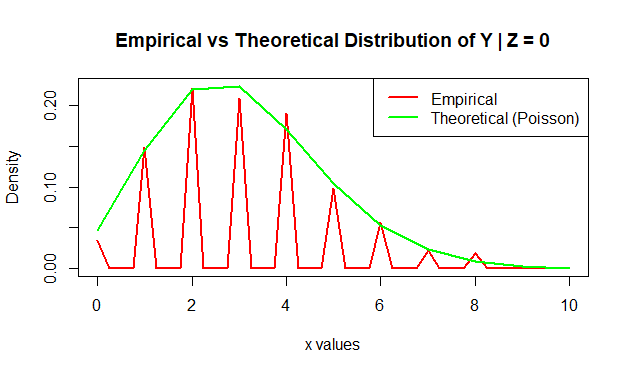
\includegraphics[width=1\linewidth]{images/Rplot07.png}
    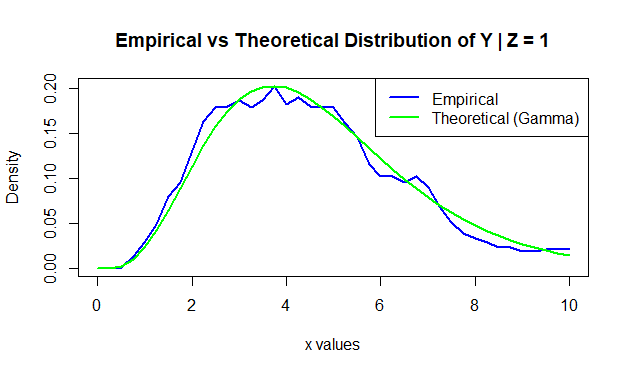
\includegraphics[width=1\linewidth]{images/Rplot08.png}
\end{center}
where the blue and red curves are the empirical densities, while the green ones are the true densities that the empirical densities are meant to reproduce.








\newpage


\section{Exercise 2}
We simulate the parameters
\[\mu \sim U(-1.5,1.5), \ \sigma^2 \sim U(0.5,1.5)\]
obtaining the values
\[ \mu = 0.706901281373575,\ \sigma^2 = 1.02490245504305.\]
We have a random variable \(X \in [0,1]\) following a \textit{logistic-normal} distribution, whose density is
\[ f(x|\mu,\sigma^2) = \frac{1}{x(1-x)} \frac{1}{\sqrt{2\pi\sigma^2}} \exp \left(-\frac{(logit(x)-\mu)^2}{2\sigma^2} \right)\]
where
\[logit(x) = \log \left( \frac{x}{1-x}\right).\]


\subsection{Data simulation with the Accept-Reject method}


In order to simulate a set of \(n = 10\) data points from the \textit{logistic-normal}, we simulate a much larger number of samples, in our case \(n^* = 1000\), from a random variable \(U \sim U(0,M)\), where \(M = 1.972316\) is the maximum value attained by the density at hand over its support; the generated values are the samples of the density that we have to accept or reject. \\ We then simulate \(n^*\) samples from a random variable \(Y \sim U(0,1)\), which are the abscissae corresponding to the samples previously generated from \(U\), and in a vector \(X\) we store only those samples generated from \(Y\) whose indices correspond to the indices of the samples generated from \(U\) that satisfy, denoting by \(u\) the generic sample generated from \(U\) and by \(x^*\) the generic sample generated from \(Y\), the condition \(u < f(x^*|\mu,\sigma^2)\). \\
Analogously, in a vector \(U\_X\) we store the samples generated from \(U\) that satisfy the condition \(u < f(x^*|\mu,\sigma^2)\). \\
We will therefore have stored in the vector \(U\) the \(n^*\) samples of the simulation of the density function, with the corresponding abscissae in \(Y\), while the accepted samples, which correctly describe the \textit{logistic-normal} density, are contained in \(U\_X\) and the corresponding abscissae in \(X\). \\
The acceptance rate of the \textit{accept-reject} method is in this case
\[perc\_acceptance = 0.51.\]
The theoretical support for these operations is provided by the following:

\begin{theorem}
    Simulating \(X \sim f(x)\), where \(X\) is defined on an arbitrary domain, is equivalent to simulating
    \[(X,U) \sim U\{(x,u): 0 < u < f(x)\}\]
    i.e. \((X,U)\) is uniform on \(\{(x,u): 0 < u < f(x)\}\).
\end{theorem}

Since we are asked to select \(n = 10\) data points, we keep only the first 10 elements of each vector, obtaining the following results:
\begin{center}
    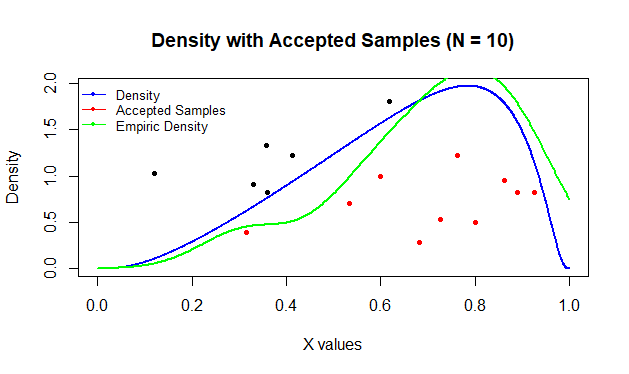
\includegraphics[width=1\textwidth]{images/Rplot.png}
\end{center}
where the blue curve is the density of the \textit{logistic-normal}, the black dots are the rejected samples, the red dots the accepted ones and the green curve the empirical density of the accepted samples. \\
Given the small number of accepted samples \(n = 10\), the empirical density does not describe correctly the density of the \textit{logistic-normal}; indeed, obtaining a more accurate empirical density would require increasing the number of accepted samples.







\subsection{Derivation of the posterior and direct sampling}
We derive the posterior starting from a prior \( \mu \sim N(0,100)\) and \(\sigma^2\) known and equal to the value used in the previous point. \\
We apply the following:
\begin{theorem}[Bayes]
    Given a parameter \(\theta\) and a finite set of observations \((x_1,...,x_n)\), we obtain
    \[ \pi(\theta|x_1,...,x_n) = \frac{\pi(\theta)L(\theta|x_1,...,x_n)}{f(x_1,...,x_n)}\]
    where \(f(x_1,...,x_n)\) is the marginal distribution of the data, \(\pi(\theta|x_1,...,x_n)\) is the posterior distribution of \(\theta\), \(\pi(\theta)\) the prior distribution of \(\theta\) and \(L(\theta|x_1,...,x_n)\) the likelihood of the parameter \(\theta\) with respect to the observations \((x_1,...,x_n)\).
\end{theorem}
Since \(\pi(\theta|x_1,...,x_n)\) is a function of \(\theta\), it follows that
\[\pi(\theta|x_1,...,x_n) \propto \pi(\theta)L(\theta|x_1,...,x_n).\]
In our case the parameter \(\theta\) is \(\mu \sim N(0,100)\), hence:
\begin{align*}
    \pi(\mu|x_1,...,x_n) &\propto L(\mu|x_1,...,x_n)\pi(\mu) \\
    &= \left(\prod_{i=1}^{n} \frac{1}{x_i(1-x_i)} \frac{1}{\sqrt{2\pi\sigma^2}} \exp \left(-\frac{(logit(x_i)-\mu)^2}{2\sigma^2} \right) \right) \left( \frac{1}{\sqrt{200 \pi}} \exp\left(-\frac{\mu^2}{200} \right) \right)  \\
    &\propto \left(\prod_{i=1}^{n} \exp \left(-\frac{(logit(x_i)-\mu)^2}{2\sigma^2} \right)  \right) \exp\left(-\frac{\mu^2}{200} \right) \\
    &= \exp \left( -\frac{1}{2\sigma^2}\sum_{i=1}^{n} (logit(x_i)^2 - 2\mu  logit(x_i) + \mu^2) \right) \exp\left(-\frac{\mu^2}{200} \right) \\
    &\propto \exp \left( - \frac{1}{2\sigma^2} \left( n\mu^2 - 2\mu \sum_{i=1}^{n} logit(x_i) + \frac{\sigma^2 \mu^2}{100}\right) \right) \\
    &= \exp \left( - \frac{1}{2\sigma^2} \left( \mu^2\left( n + \frac{\sigma^2}{100} \right)- 2\mu \sum_{i=1}^{n} logit(x_i)\right) \right) \\
    &\propto \exp \left( - \frac{1}{2} \frac{\left(n + \frac{\sigma^2}{100} \right)}{\sigma^2} \left( \mu^2- \frac{2\mu \sum_{i=1}^{n} logit(x_i)}{\left(n + \frac{\sigma^2}{100} \right)} + \left( \frac{(\sum_{i=1}^{n} logit(x_i))^2}{\left(n + \frac{\sigma^2}{100} \right)^2} \right)\right) \right) \\
    &= \exp \left(- \frac{1}{2} \frac{\left( \mu - \frac{\sum_{i=1}^{n} logit(x_i)}{n+\frac{\sigma^2}{100}} \right)^2}{\frac{\sigma^2}{n + \frac{\sigma^2}{100}}} \right)
\end{align*}

which is the \textit{kernel} of a \(N\left( \frac{\sum_{i=1}^{n} logit(x_i)}{n+\frac{\sigma^2}{100}},  \frac{\sigma^2}{n + \frac{\sigma^2}{100}}\right)\) distribution, from which we deduce that
\[\pi(\mu|x_1,...,x_n) \sim N\left( \frac{\sum_{i=1}^{n} logit(x_i)}{n+\frac{\sigma^2}{100}},  \frac{\sigma^2}{n + \frac{\sigma^2}{100}}\right).\]
We have therefore obtained that the posterior follows a known distribution, namely a \textit{normal} one, from which it is possible to sample directly. \\
In order to represent the posterior graphically, we consider the abscissae of the accepted samples from the \textit{logistic-normal} contained in \textit{X}. The results are shown in the following histogram:
\begin{center}
    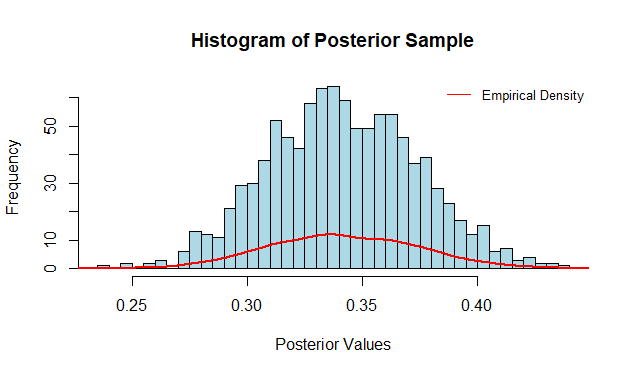
\includegraphics[width=1\textwidth]{images/Rplot01.png}
\end{center}
where the horizontal axis reports the values taken by the posterior and the vertical axis the frequency with which they are taken. The red line is the empirical density of those values.

\subsection{Comparison between \textit{prior} and \textit{posterior}}
Using the method described above, we select the first \(n_2 = 100\) elements of each vector used in the \textit{accept-reject} sampling, so as to obtain a simulation of \(n_2 = 100\) samples from the \textit{logistic-normal}. We compare them with the \(n_1 = 10\) samples computed before, obtaining the following results:
\begin{center}
    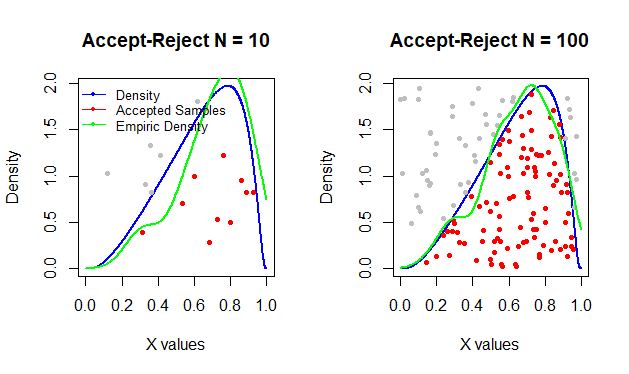
\includegraphics[width=1\textwidth]{images/Rplot02.png}
\end{center}
that is, a more accurate simulation on the right, using \(n_2 = 100\) samples. \\
Now, out of both the \(n_1 = 10\) and the \(n_2 = 100\) accepted samples \(u\_x_1\) and \(u\_x_2\) we select the abscissae, contained in the vectors \textit{X10\_sample} and \textit{X100\_sample}, and we use these values to simulate from the posterior, obtaining the following results:
\begin{center}
    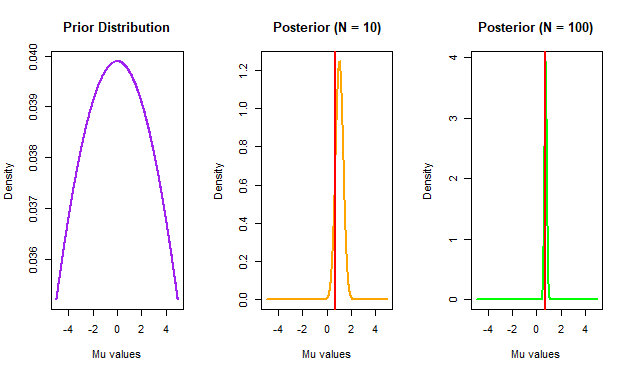
\includegraphics[width=1\textwidth]{images/Rplot03.png}
\end{center}
where on the left we have the prior distribution of the parameter \(\mu\), in the centre the posterior distribution using the set of \(n_1 = 10\) samples as observations, on the right the posterior distribution using the set of \(n_2 = 100\) samples as observations, while the vertical red line marks the actual value of the parameter \(\mu\). \\
As expected from the theory, the posterior distribution conditional on the \(n_1 = 10\) observations turns out to be \textit{wider} than the one conditional on the \(n_2 = 100\) observations, which is centred on the actual value of the parameter \(\mu\). \\



\subsection{Computation of the mean with the Importance-Sampling method}
We are asked to compute
\[E(X) = \int_{\mathcal{X}} x f(x) \ d\lambda(x)\]
where \(f(x)\) is the density of the \textit{logistic-normal} distribution.\\
Denoting by \(g(x)\) the density of a \textit{beta} distribution with parameters \(a = 1.2 \) and \(b = 1.2\), this integral can be rewritten as
\[E(X) = \int_{\mathbf{\mathcal{X}}} x f(x) \ d\lambda(x) = \int_{\mathcal{X}} \frac{x f(x)}{g(x)} g(x) \ d\lambda(x) = E_g\left(\frac{Xf(X)}{g(X)}\right).\]
If \(x_i,\ i = 1,...,n,\) are samples obtained from the \textit{beta} distribution with density \(g\), we have that
\[E_g\left(\frac{Xf(X)}{g(X)}\right) \approx \frac{\sum_{i = 1}^{n}\frac{x_i f(x_i)}{g(x_i)}}{n}.\]
We set \(n = 1000\), we sample directly from the \textit{beta}, obtaining \(n = 1000\) observations, and we use the approximation above, obtaining the following results:
\begin{center}
    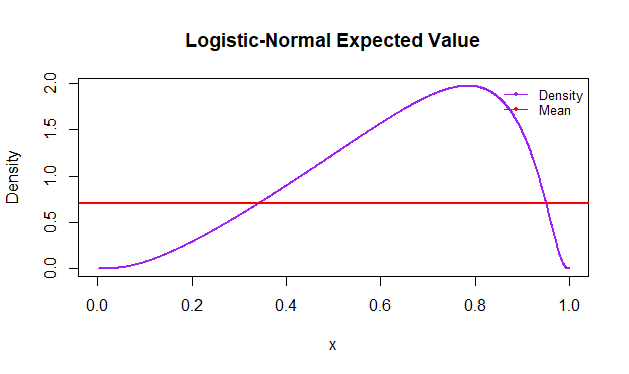
\includegraphics[width=1\textwidth]{images/Rplot04.png}
\end{center}
where the purple curve is the density of the \textit{logistic-normal} and the red line the expected value of that density, computed with the Importance-Sampling method. \\
The value obtained from the estimate is
\[E(X) \approx 0.6373222.\]

\end{document}
